\section{Auswertung}
\label{sec:Auswertung}

\subsection{Untersuchung der Filterkurve}

Für die Filterkurve wurden die folgenden \autoref{tab:tab1} Messadaten aufgenommen, dabei wurde eine 10-fache Verstärkung verwendet.

\begin{table}[H]
    \centering
    \caption{Messwerte zur Filterkurve.}
    \label{tab:tab1}
    \begin{tabular}{S S}
      \toprule
      {$f \mathbin{/} \unit{\kilo\hertz} $} & {$U \mathbin{/} \unit{\milli\volt} $}  \\
      \midrule
            10.01       &   0.5     \\
            12.95       &   0.78    \\
            16.03       &   1.11    \\
            19.03       &   2.73    \\
            20.1        &   4.4     \\
            21.0        &   8.1     \\
            22.7        &   6.9     \\
            21.1        &   8.1     \\
            30.6        &   0.84    \\
            33.0        &   0.6     \\
            36.2        &   0.51    \\
            38.3        &   0.46    \\
            40.0        &   0.4     \\
      \bottomrule
    \end{tabular}
\end{table}

Die Messwerte aus \autoref{tab:tab1} sind auch in \autoref{fig:Graph_a} dargestellt.

\begin{figure}[H]
    \centering
    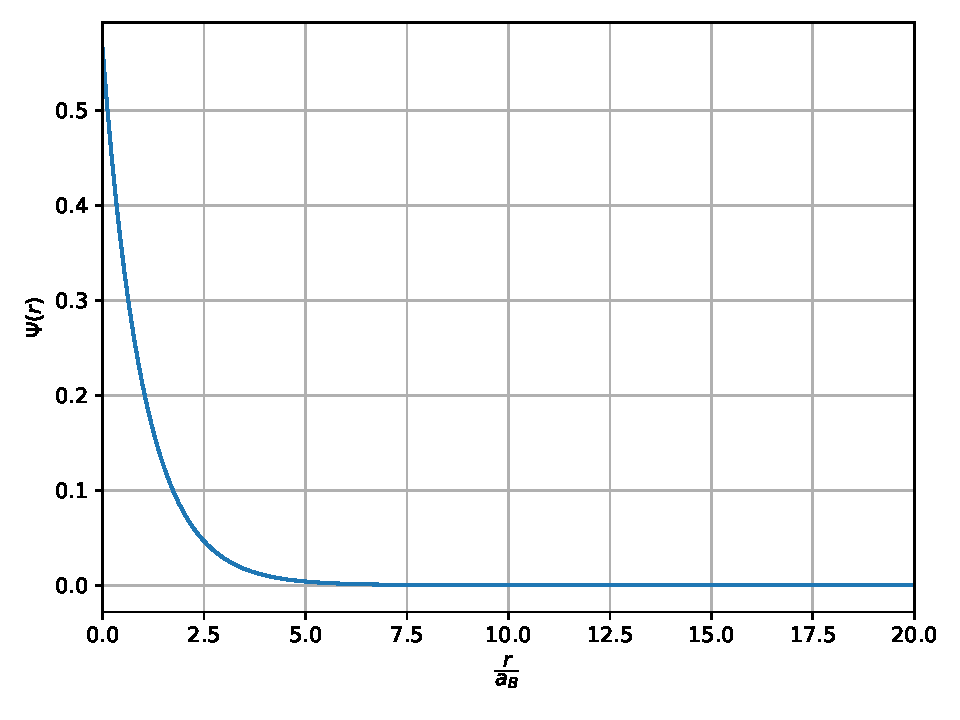
\includegraphics{build/Graph_a.pdf}
    \caption{Filterkurve der Brückenschaltung}
    \label{fig:Graph_a}
\end{figure} 

Es wurde versucht mit $ scipy$ eine Lorentzkurve der Form \eqref{eq:Lorentzkurve}, sowie eine Gaußverteilung der Form \eqref{eq:gauß} zu fitten, jedoch konnten keine Parameter, die zu den Messdaten passen gefunden werden

\begin{equation}
    f_l(v) = \frac{a}{(v^2-v_0^2)^2 + {\gamma}^2 v_0^2}
    \label{eq:Lorentzkurve}
\end{equation}

\begin{equation}
    f_g(v) = b \cdot \exp{\frac{(v-v_0)^2}{a}} \,.
    \label{eq:gauß}
\end{equation} 

Das Maximum der Spannung wird als

\begin{equation}
    U_\text{A} = 8,1 \, \unit{\volt}
\end{equation}

bei einer Frequenz von 
\begin{equation}
    v_0 = 21,05 \, \unit{\kilo\hertz}
\end{equation}
bestimmt.

\subsection{Bestimmung der Suszeptibilität}

Um einen besseren Überblick über die Qualität der aufgenommenen Messwerte zu erhalten, ist es sinnvoll, diese mit den theoretisch berechneten Suszeptibilitäten zu vergleichen.
Dabei wird nach den Hundschen Regeln vorgegangen. \\

Zu beachten ist dabei auch die Orientierungsquantenzahl $m = (-3, \,-2, \,-1, \,0, \,1, \,2, \,3)$, die für Elektronen mit gleichem Spin immer unterschiedlich sein muss.
Für die drei Proben folgt also:

\begin{itemize}
    \item $\text{Nd}_2 \text{O}_3$ besitzt auf der 4f-Schale drei Elektronen, die nach der ersten Hundschen Regel den gleichen Spin $s_\text{i} = \frac{1}{2}$, also kombiniert einen Gesamtspin von $S = \frac{3}{2}$ besitzen.
          Die drei Elektronen müssen sich also in ihrer Orientierungsquantenzahl unterscheiden. 
          Hier folgt ein maximaler Drehimpuls von $L = \sum m_i = 3 + 2 + 1 = 6$, insgesamt also ein Gesamtdrehimpuls von $J = L - S = 6 - \frac{3}{2} = \frac{9}{2}$,
          da die Schale weniger als halb gefüllt ist.
          Damit ergibt sich nach \eqref{eq:lande-faktor} ein Landé-Faktor von $g_\text{J} = \frac{8}{11}$.

    \item Für $\text{Gd}_2\text{O}_3$ wird analog vorgegangen. Mit sieben Elektronen auf der 4f-Schale mit gleichem Spin folgt $S = 3,5$. 
        Da die Anzahl an Elektronen genau gleich der Anzahl unterschiedlicher Orientierungsquantenzahlen ist, ist der Bahndrehimpuls $L = 0$.
        Der Gesamtdrehimpuls ist damit gleich dem Gesamtspin, $J = S = 3,5$ und der Landé-Faktor $g_\text{J} = 2$.

    \item Mit neun Elektronen auf der 4f-Schale besitzt $\text{Dy}_2\text{O}_3$ mehr Elektronen, als es Orientierungsquantenzahlen gibt, zwei der Elektronen haben also einen negativen Spin.
        Damit ergibt sich $S = 2,5$ und ein Bahndrehimpuls von \\ $L = 3 + 2 + 1 + 0 - 1 - 2 - 3 + 3 + 2 = 5$.
        Für den Gesamtdrehimpuls folgt $J = L + S = 7,5$, da die Schale mehr als halb gefüllt ist, für den Landé-Faktor $g_\text{J} = \frac{4}{3}$.
\end{itemize}

Mit der Avogadrokonstanten $N_a$, der Dichte $\rho$ und der molaren Masse $M_\text{mol}$ gilt für die Anzahl der Momente pro Volumen
\begin{equation}
    N = 2 N_a \dfrac{\rho}{M_\text{mol}} \,,
\end{equation}
womit sich nach \eqref{eq:susg_J} und den in \autoref{tab:probwertis} aufgetragenen Dichten, molaren Massen sowie der berechneten Anzahl der Momente pro Volumen
die in \autoref{tab:theosus} dargestellten theoretischen Suszeptibilitäten ergeben.

\begin{table}[H]
    \centering
    \caption{Dichten $\rho$, molare Massen $M_\text{mol}$ und berechnete Momente pro Volumen $N$.}
    \label{tab:probwertis}
    \begin{tabular}{S S[table-format=1.2] S[table-format=3.2] S[table-format=1.2]}
      \toprule
      {} & {$\rho \mathbin{/} \unit{\frac{\gram}{{\centi\meter}^3}}$} & {$M_\text{mol} \mathbin{/} \unit{\frac{\gram}{\mol}}$} & {$N \mathbin{/} \unit{\frac{1}{{\centi\meter}^3}} \cdot 10^{28}$}  \\
      \midrule
      {$\text{Nd}_2 \text{O}_3$}        &           7.24          &         336.48          &           2.59            \\
      {$\text{Gd}_2\text{O}_3$}         &           7.40          &         362.50          &           2.46            \\
      {$\text{Dy}_2\text{O}_3$}         &           7.80          &         373.00          &           2.52            \\
      \bottomrule
    \end{tabular}
\end{table}

\begin{table}[H]
    \centering
    \caption{Theoretische Suszeptibilitäten $\chi_\text{theo}$ der unterschiedlichen Proben.}
    \label{tab:theosus}
    \begin{tabular}{S S[table-format = 1.6]}
      \toprule
      {} & {$\chi_\text{theo}$}  \\
      \midrule
      {$\text{Nd}_2 \text{O}_3$}        &           0.00299         \\
      {$\text{Gd}_2\text{O}_3$}         &           0.01370         \\
      {$\text{Dy}_2\text{O}_3$}         &           0.02525         \\
      \bottomrule
    \end{tabular}
\end{table}